\documentclass[tikz,convert={outext=.svg,command=\unexpanded{pdf2svg \infile\space\outfile}},multi=false]{standalone}
\usepackage[utf8]{inputenc}

\begin{document}


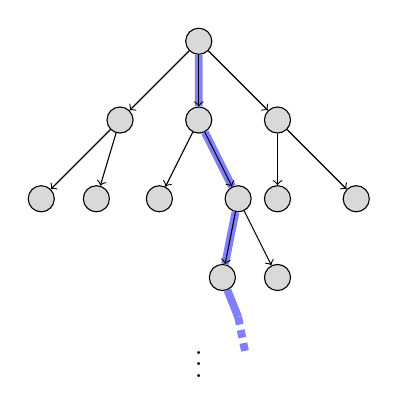
\begin{tikzpicture}
\tikzstyle{noeud}=[draw, circle, fill=gray!30!white];
\tikzstyle{branche}=[line width=1mm, blue!50!white];
\node[noeud] (epsilon) at (0, 0) {};
\node[noeud] (0) at (-1,-1) {};
\node[noeud] (1) at (0,-1) {};
\node[noeud] (2) at (1,-1) {};
\node[noeud] (00) at (-2,-2) {};
\node[noeud] (01) at (-1.3,-2) {};
\node[noeud] (11) at (-0.5,-2) {};
\node[noeud] (12) at (0.5,-2) {};
\node[noeud] (20) at (1,-2) {};
\node[noeud] (21) at (2,-2) {};
\node[noeud] (120) at (0.3,-3) {};
\node[noeud] (121) at (1,-3) {};

\draw[branche] (epsilon) -- (1) -- (12) -- (120);
\draw[branche] (120) -- (0.5, -3.5) edge[dotted] (0.6, -4);

\draw[->] (epsilon) edge (0);
\draw[->] (epsilon) edge (1);
\draw[->] (epsilon) edge (2);
\draw[->] (0) edge (00);
\draw[->] (0) edge (01);
\draw[->] (1) edge (11);
\draw[->] (1) edge (12);
\draw[->] (2) edge (20);
\draw[->] (2) edge (21);
\draw[->] (12) edge (120);
\draw[->] (12) edge (121);
\node at (0, -4) {$\vdots$};
\end{tikzpicture}
\end{document}